\Class{Gladiator}
{I might be a slave, but I am famous, I dine well, and my company is that of the finest noble women. Tell me, what do you have that I do not, slave trader---except the freedom to feel miserable?}{Jarek, arena champion}

\begin{figure}[t!]
\centering
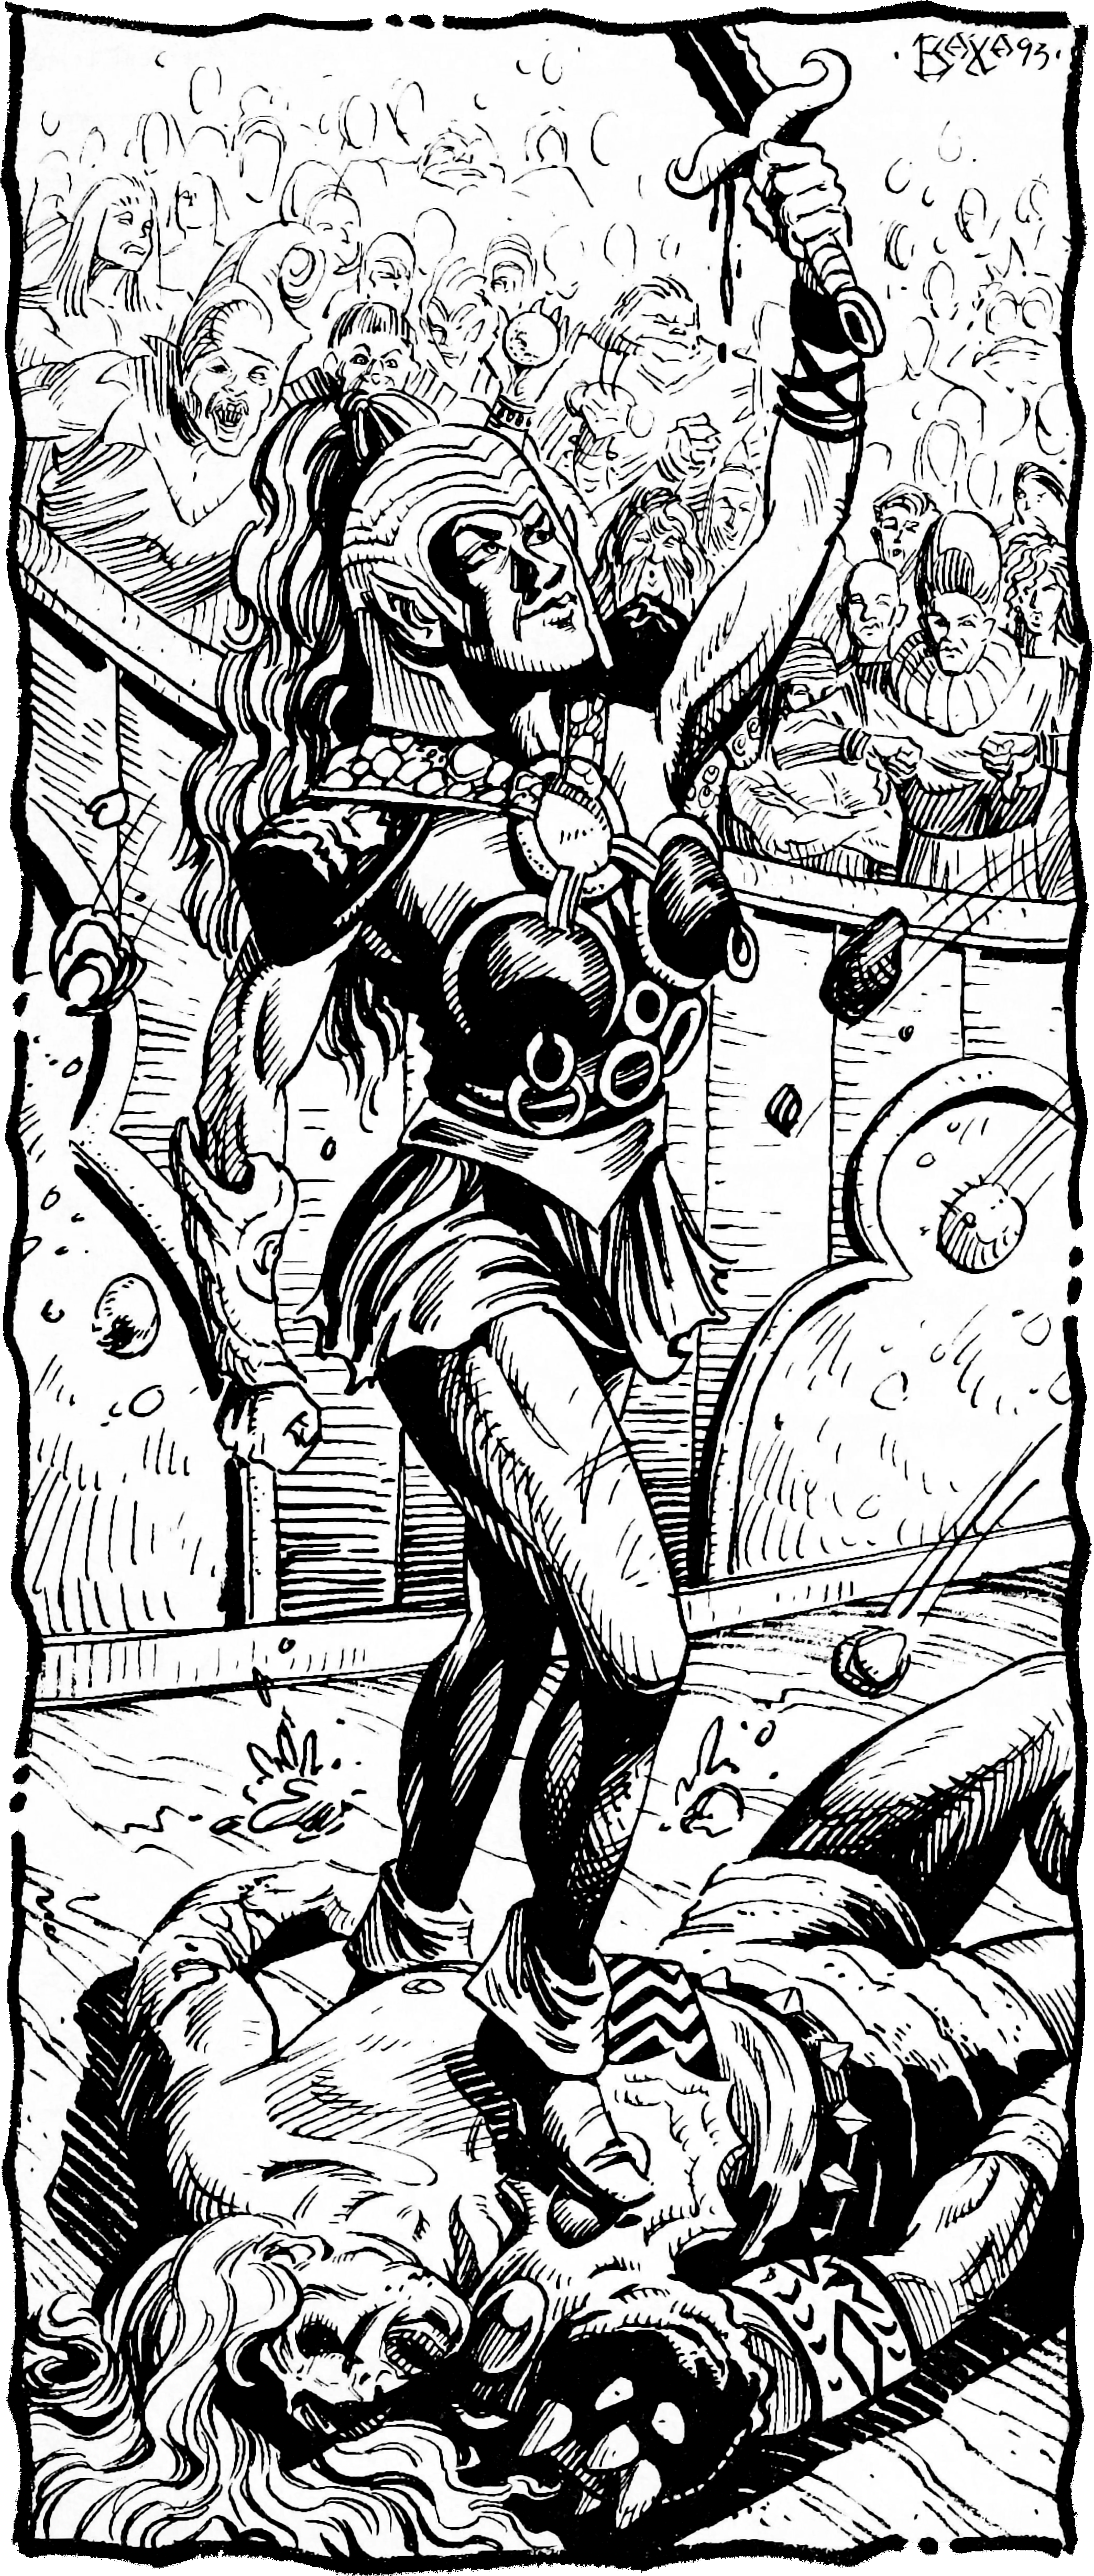
\includegraphics[width=\columnwidth]{images/gladiator-2.png}
\WOTC
\end{figure}

The arena is the battlefield of the gladiator. From hand-to-hand combat in the mud pits of small forts to the grand games of the city-states, the gladiator is a warrior who fights to the sounds of people cheering his name or cursing his presence. A master of crowd control and the art of prolonged combat, gladiators are trained to fight.

They train to best wild beasts in deadly games for the amusement of the masses. They fight for glory, wealth, prestige and power. They fight to survive. Some are merely slaves, having to fight and perhaps hoping to win a chance to obtain freedom, while some fight willingly for the thrill of combat or the promise of riches and fame.

\WarriorTable[ll *{3}{C} p{8cm}]{The Gladiator}{
1st  & +1             & +2  & +0 & +0 & Unarmed strike, gladiatorial performance, dirty trick $\pm2$/$\pm4$                 \\
2nd  & +2             & +3  & +0 & +0 & Bonus feat, exotic weapon, stance (arena guile)                                     \\
3rd  & +3             & +3  & +1 & +1 & Bonus feat, exotic aptitude, taunt                                                  \\
4th  & +4             & +4  & +1 & +1 & Uncanny dodge                                                                       \\
5th  & +5             & +4  & +1 & +1 & Armor optimization 1, \feat{Improved Feint}                                         \\
6th  & +6/+1          & +5  & +2 & +2 & Exotic weapon, parry, shake off                                                     \\
7th  & +7/+2          & +5  & +2 & +2 & Bonus feat, dirty trick $\pm4$/$\pm6$, stance (threatening glare, defensive stance) \\
8th  & +8/+3          & +6  & +2 & +2 & Improved uncanny dodge, mercy                                                       \\
9th  & +9/+4          & +6  & +3 & +3 & \feat{Leadership}, pounce                                                           \\
10th & +10/+5         & +7  & +3 & +3 & Armor optimization 2, exotic weapon                                                 \\
11th & +11/+6/+1      & +7  & +3 & +3 & Improved parry                                                                      \\
12th & +12/+7/+2      & +8  & +4 & +4 & Dragon's fury, stance (keen eye, scoundrel pose)                                    \\
13th & +13/+8/+3      & +8  & +4 & +4 & Dirty trick $\pm6$/$\pm8$, greater feint                                            \\
14th & +14/+9/+4      & +9  & +4 & +4 & Exotic weapon                                                                       \\
15th & +15/+10/+5     & +9  & +5 & +5 & Armor optimization 3, dragon's speed                                                \\
16th & +16/+11/+6/+1  & +10 & +5 & +5 & Greater parry                                                                       \\
17th & +17/+12/+7/+2  & +10 & +5 & +5 & Stance (balancing dance, hypnotic fortitude)                                        \\
18th & +18/+13/+8/+3  & +11 & +6 & +6 & Exotic weapon, mindless focus                                                       \\
19th & +19/+14/+9/+4  & +11 & +6 & +6 & Dirty trick $\pm8$/$\pm10$                                                          \\
20th & +20/+15/+10/+5 & +12 & +6 & +6 & Armor optimization 4                                                                \\
}


\subsection{Making a Gladiator}
Gladiators are among the best one-on-one fighters in all the Tablelands. They are trained in hand-to-hand combat before moving on to the use of exotic weapons of the arena. They learn to improvise weapons, wielding broken bones or wooden shafts with deadly precision. They learn how to taunt and tease opponents, driving them to reckless acts and taking advantage of the situation to strike down or maim a foe.

After all, a long, drawn-out combat is more a crowd pleaser than a ten-second bout.

\textbf{Abilities:} Strength and Constitution are vital to a gladiator, since he is often in harm's way. Intelligence is useful for gaining plenty of skills points, which a gladiator needs to purchase Bluff, Intimidate, Performance, and Sense Motive, key skills for any arena performer.

\textbf{Races:} All races of Athas can be found in the arenas of the Tablelands. Muls, with their mixed dwarven and human parentage, are highly prized in the arenas. They are often bought for a high price and treated well in return for victory on the combat floor. Elves are often used for their swiftness and natural flair for taunting their opponent. Humans are the most common of gladiators, since humans are the most common race in the Tablelands. Halflings make poor gladiators, since they abhor slavery and will usually starve themselves to death rather than being used as commodities by anyone. The savage races of the wastes are often used as gladiators, usually as fodder for the most successful gladiators, though those demonstrating excellent combat prowess receive formal training.

\textbf{Alignment:} Gladiators are of all alignments. Some gladiators will obey all arena rules, being lawful individuals, though these often do not last long in the arena. Many gladiators tend toward a chaotic alignment. Evil gladiators use dirty tricks to gain an advantage over an opponent. Gladiators of all alignments can become crowd favorites, increasing their chances of winning their matches, since often times these matches are prearranged. The intrigues of the city-states can reach deep into the arena.

\subsection{Game Rule Information}

\textbf{Hit Die:} d10.

\subsubsection{Class Skills}
\skill{Autohypnosis} (Wis), \skill{Balance} (Dex), \skill{Bluff} (Cha), \skill{Climb} (Str), \skill{Craft} (Int), \skill{Handle Animal} (Cha), \skill{Intimidate} (Cha), \skill{Jump} (Str), \skill{Perform} (Cha), \skill{Profession} (Wis), \skill{Ride} (Dex), \skill{Sense Motive} (Wis), \skill{Spot} (Wis), and \skill{Tumble} (Dex).

\textbf{Skill Points per Level:} 4 + Int modifier ($\times4$ at 1st level).

\subsubsection{Class Features}

\textbf{Weapon and Armor Proficiency:} You are proficient with all simple and martial weapons, light armor, medium armor and shields (except tower shields).

\textbf{Gladiatorial Performance:} Once per day per gladiator level, you can use your talents to affect enemies and allies. Each ability requires both a minimum gladiator level and a minimum number of ranks in the \skill{Perform} (arena fighting) skill to qualify. Starting a gladiatorial performance effect is a move action unless otherwise stated.

\textit{Dirty Trick (Ex):} A gladiator with 3 or more ranks in \skill{Perform} (arena fighting) can use his arena guile to get an advantage over his enemies. Once per encounter per opponent, a gladiator can use a dirty trick to do one of the following:

\begin{itemize*}
\item Gain +2 circumstance bonus on his attack rolls for one round per gladiator level.
\item Gain +4 circumstance bonus on his damage rolls for one round per gladiator level.
\item Impose $-2$ circumstance penalty on target opponent's attack rolls for one round per gladiator level.
\item Impose $-4$ circumstance penalty on target opponent's damage rolls for one round per gladiator level.
\end{itemize*}

A gladiator can use dirty trick more than once per encounter, but a gladiator may never repeat the same option against the same enemy or use it more than once in a single round against the same enemy. Using a dirty trick is a free action.

These bonuses and penalties increase by 2 at 7th level and every six levels thereafter ($\pm4$/$\pm6$ at 7th, $\pm6$/$\pm8$ at 13th, and $\pm8$/$\pm10$ at 19th).

\textit{Taunt (Ex):} A gladiator of 3rd level or higher with 6 or more ranks in \skill{Perform} (arena fighting) can taunt one opponent to fly into a rage. The opponent to be taunted must be within 9 meters, able to see and hear the gladiator, and must have an Intelligence of 3 or higher. The gladiator must also be able to see the creature. For every three levels a gladiator attains beyond the 1st, he can target one additional creature with a single use of this ability.

A gladiator makes a \skill{Perform} (arena fighting) check. His check result is the DC for each affected creature's Will save against the effect. If a creature's saving throw succeeds, the gladiator cannot attempt to taunt that creature again for 24 hours. If its saving throw fails, the creature flies into a blind rage. While enraged, a target takes $-2$ penalty on attack rolls and AC. The rage lasts until either the gladiator or his target become unconscious.

Taunt is a mind-affecting ability.

\textit{Shake Off (Ex):} A gladiator of 6th or higher level with 9 or more ranks in \skill{Perform} (arena fighting) can try to end a mind-affecting effect in play on himself or an ally. He shakes his head violently to clear his mind, or slap an ally to bring them back to them senses. The recipient of the shake off can reroll a single failed save or opposed skill check (with the same DC as the failed roll) to end a mind-affecting effect. If there is no save or check to avoid the mind-affecting effect, the effect ends automatically.

\textit{Pounce (Ex):} A gladiator of 9th or higher level with 12 or more ranks in \skill{Perform} (arena fighting) can throw himself with pure savagery. As a swift action, he gains the pounce ability until the end of turn, allowing the gladiator to make a full attack at the end of a charge.

\textit{Dragon's Fury (Ex):} A gladiator of 12th or higher level with 15 or more ranks in \skill{Perform} (arena fighting) can enter a trance-like state in which his full offensive gladiatorial potential is unleashed. As a full-round action, the gladiator can make a full attack with +4 competence bonus to attack rolls and damage rolls, and an additional attack made at his highest base attack bonus.

\textit{Dragon's Speed (Ex):} A gladiator of 15th or higher level with 18 or more ranks in \skill{Perform} (arena fighting) can exert himself to move more than what seems possible. As a swift action, the gladiator gains an additional move action until the end of his turn. This means that he can make use of up to three move actions in the same turn, or two move actions and a standard action, or one move action and a full-round action.

\textit{Mindless Focus (Ex):} A gladiator of 18th or higher level with 21 or more ranks in \skill{Perform} (arena fighting) may become fearless as the Dragon. As a swift action, the gladiator becomes immune to enchantment, telepathy, and mind-affecting effects until the start of his next turn. If the gladiator is already under the effect of any enchantment, telepathy, or mind-affecting effect, he may roll a \skill{Perform} (arena fighting) check against the DC of the effect to end it, instead.

\textbf{Unarmed Strike:} A gladiator gains \feat{Improved Unarmed Strike} as a bonus feat. A gladiator's attacks may be with either fist interchangeably or even from elbows, knees, and feet. This means that a gladiator may even make unarmed strikes with his hands full. There is no such thing as an off-hand attack for a gladiator striking unarmed. A gladiator may thus apply his full Strength bonus on damage rolls for all his unarmed strikes.

Usually a gladiator's unarmed strikes deal lethal damage, but he can choose to deal nonlethal damage instead with no penalty on his attack roll. He has the same choice to deal lethal or nonlethal damage while grappling.

A gladiator also deals more damage with his unarmed strikes than a normal person would. A Medium gladiator deals 1d6 points of damage. Small gladiators deal 1d4 points of damage, and Large gladiators deal 1d8 points of damage.

\textbf{Stance (Ex):} Starting at 2nd level, a gladiator may adopt a combat stance. Each stance requires a minimum gladiator level and a minimum number of ranks in a skill. A gladiator assumes a stance as a swift action. A stance remains in effect indefinitely and is not expended. He enjoys the benefit his stance confers until he changes to another stance he knows as a swift action. He can remain in a stance outside of combat situations, and he can enjoy its benefit while exploring or traveling.

\textit{Arena Guile (Ex):} A gladiator of 2nd level or higher may add one-half his gladiator level (rounded down) as a bonus to all \skill{Bluff} and \skill{Sense Motive} checks that relate directly to melee combat.

% \textit{Shorten Haft (Ex):} A gladiator of 7th level or higher with 10 or more ranks in \skill{Balance} may use reach weapons with greater prowess. He threatens adjacent squares when wielding reach weapons. A gladiator cannot use this stance if he is being flanked. 

\textit{Threatening Glare (Ex):} A gladiator of 7th level or higher with 10 or more ranks in \skill{Intimidate} may cause fear into his enemies when fighting with a group. If both him and an ally are adjacent and threatening the same creature, the two of them gain the benefit for flanking that opponent. The gladiator can gain this benefit against multiple opponents at the same time, as can his allies. If both him and an ally are adjacent and threatening the same two creatures, the two of them gain the benefit of flanking against both creatures. A gladiator cannot use this stance if he is wielding a two-handed weapon.

\textit{Defensive Stance (Ex):} A gladiator of 7th level or higher with 10 or more ranks in \skill{Tumble} can improve his defenses when fighting defensively or in total defense. When in total defense, he may add \onehalf his gladiator level as dodge bonus to AC. When fighting defensively, he may add \onequarter his gladiator level as dodge bonus to AC. A gladiator cannot use this stance if he is wearing medium armor or heavier.

\textit{Keen Eye (Ex):} A gladiator of 12th level or higher with 15 or more ranks in \skill{Spot} may find weakness in the enemies defenses. Whenever he misses an attack, he gains a circumstance bonus on the next attack equal to +2 for each previous miss in the same round. While in this stance, as a swift action the gladiator may expend two of his daily gladiatorial performances to ignore armor bonus and natural bonus on a single attack. 

\textit{Scoundrel Pose (Ex):} A gladiator of 12th level or higher with 15 or more ranks in \skill{Bluff} can fool lesser enemies and back stab. He is treated as if he had a rogue level equal to his gladiator level $-2$, so he can flank foes with improved uncanny dodge. While in this stance, as a swift action the gladiator may expend two of his daily gladiatorial performances to gain sneak attack +5d6 until his next turn.

% \textit{Mindless Focus (Ex):} A gladiator of 17th level or higher with 20 or more ranks in \skill{Autohypnosis} may become fearless as the Dragon. He becomes immune to fear effects. While in this stance, as a swift action the gladiator may expend one of his daily gladiatorial performances to become immune to mind-affecting abilities for one round.

\textit{Balancing Dance (Ex):} A gladiator of 17th level or higher with 20 or more ranks in \skill{Balance} gains additional reach with melee weapons. Each time he makes a successful melee attack, he can move 1.5 meter. This movement does not provoke attacks of opportunity from the creature he struck. A gladiator cannot use this stance to move more than his current speed in a single round.

\textit{Hypnotic Fortitude (Ex):} A gladiator of 17th level or higher with 20 or more ranks in \skill{Autohypnosis} can gain extraordinary resilience to endure incapacitating strikes. So long as he remains in this stance, he cannot be killed or incapacitated by effects or attacks that reduce him to 0 or fewer hit points. If he takes such damage, he can make an \skill{Autohypnosis} check with a DC equal to the damage received. If he fails this save, he dies or falls unconscious (as appropriate). If this save is successful, he is still alive and conscious, with 1 hit point remaining.

After he attempts three \skill{Autohypnosis} checks to avoid death or unconsciousness, this stance automatically ends. He can activate it again on his turn as normal. Even the toughest gladiator can endure only so much punishment.

\textbf{Bonus Feat:} At 2nd level, a gladiator may select either \feat{Blind-Fight} or \feat{Endurance} as bonus feat. At 3rd level, a gladiator may select either \feat{Combat Expertise} or \feat{Mounted Combat} as bonus feat. At 7th level, a gladiator may select one of \feat{Improved Bull Rush}, \feat{Improved Disarm}, \feat{Improved Grapple}, \feat{Improved Overrun}, \feat{Improved Sunder}, \feat{Improved Trip}, or \feat{Ride-By Attack}. A gladiator need not have any of the prerequisites normally required for these feats to select them.

\textbf{Exotic Weapon:} At 2nd level, a gladiator gains \feat{Exotic Weapon Proficiency} as a bonus feat. He gains a new exotic weapon proficiency every four levels thereafter, at 6th, 10th, 14th, and 18th level.

\textbf{Exotic Aptitude (Ex):} Beginning at 3rd level, a gladiator qualifies for feats that usually require a minimum number of fighter levels (such as \feat{Weapon Specialization}) as if he had a fighter level equal to his gladiator level $-2$. For example, a 6th-level gladiator could take \feat{Weapon Specialization}, since he's treated as being a 4th-level fighter for this purpose. These fighter levels stack with any actual fighter levels he has. Thus, a fighter 2/gladiator 4 would also qualify for \feat{Weapon Specialization}.

The gladiator may also apply any feat that applies only to a single weapon (such as \feat{Weapon Focus}) to any exotic weapon he has proficiency. For example, a 6th-level gladiator who has \feat{Weapon Focus} (longsword) and \feat{Weapon Specialization} (longsword) can also apply these feats bonus on attack and damage rolls of any exotic weapon with which he has \feat{Exotic Weapon Proficiency}.

\textbf{Uncanny Dodge (Ex):} At 4th level, a gladiator retains his Dexterity bonus to AC (if any) even if he is caught flat-footed or struck by an invisible attacker. However, he still loses his Dexterity bonus to AC if immobilized. If a gladiator already has uncanny dodge from a different class, he automatically gains improved uncanny dodge instead.

\textbf{Armor Optimization (Ex):} At 5th level, a gladiator gains an understanding of how his armor can better serve him. He increases the armor bonus to AC and reduces the armor check penalty by 1 whenever he is wearing any armor he is proficient with.

At every five levels thereafter, the improvement increases by 1 (2 at 10th, 3 at 15th, and 4 at 20th level).

\textbf{Improved Feint:} At 5th level, a gladiator gains \feat{Improved Feint} as a bonus feat.

% \textbf{No Mercy (Ex):} Beginning at 6th level, you can perform a coup de grace as a standard action rather than a full-round action.

\textbf{Parry (Ex):} Beginning at 6th level, once per round a gladiator can forfeit an attack to attempt to parry an incoming melee attack. The forfeited attack has to be the one with his highest base attack bonus. If wielding two weapons, the parry must be made using his secondary weapon. The gladiator makes an opposed attack roll with a $-5$ penalty against his attacker roll. If he succeeds, the attack is parried and he suffers no damage or ill effects related to the attack, including touch attacks used to deliver spells.

\textbf{Improved Uncanny Dodge (Ex):} At 8th level and higher, a gladiator can no longer be flanked. This defense denies a rogue the ability to sneak attack the gladiator by flanking him, unless the attacker has at least four more rogue levels than the target has gladiator levels. If a character already has uncanny dodge from a second class, the character automatically gains improved uncanny dodge instead, and the levels from the classes that grant uncanny dodge stack to determine the minimum level a rogue must be to flank the character.

\textbf{Mercy (Ex):} At 8th level, a gladiator suffers no penalty to attack rolls when attacking with a weapon to inflict nonlethal damage.

\textbf{Leadership:} At 9th level, a gladiator gains \feat{Leadership} as a bonus feat.

\textbf{Improved Parry:} At 11th level, a gladiator no longer suffer a $-5$ penalty to his opposed attack roll for parry.

\textbf{Greater Feint:} Beginning at 13th level, a gladiator can make a \skill{Bluff} check to feint in combat as a free action.

\textbf{Greater Parry:} At 16th level, a gladiator may forfeit two attacks to parry, instead of one. Both forfeited attacks must be the ones with highest base attack bonus. If wielding two weapons, both parries must be made using his secondary weapon.

\subsection{Playing a Gladiator}
Mastering the techniques of blade and shield is important to you, but even more is the sense of daring, danger, and even joy that you feel when you battle inside the arena. You fight for the glory, the thrill of combat, and for the adoration of the crowd. Thus, you approach each encounter as if the bards will sing of it for ages. Silver and concubines are pleasant tokens, but the real measure of your success is how loud the crowd screams your name when you step into the pit.

As a gladiator, you find adventure wherever an opportunity for glory exists. You might be one of the gladiators that went out of job when the sorcerer-king of you city was killed by Tyrians and now you have become a mercenary warrior, still looking for the thrill of combat. You might have been able to flee from your owner and now user your sword to protect your slave tribe.

\subsubsection{Religion}
Gladiators have no special religion of their own. Some may worship the sorcerer-king of the city-state they are in, while some few may worship the elemental forces. Often, the hard life of training and combat leaves the gladiator with little to think of except survival.

\subsubsection{Other Classes}
Gladiators tend to think of themselves as the superior warriors of the Tablelands, sometimes to the point of arrogance.

In a sense, though, they are right. Gladiators receive training in one-on-one combat, and the use of anything they can find as a weapon. However, a group of trained fighters fighting in concert is certainly a match for a bunch of gladiators, who are unused to fighting in groups. Like most people of Athas, gladiators have a deep distrust of magic, and tend to shun wizards. They view clerics as nothing more than healers, people who put their faith in abstract things rather than a sharp blade.

\subsubsection{Combat}
You revel in melee. Your place is battling against hulking baazrags and wicked tembo, where you can hear the crowd cheering and chanting your name. You make good use of your various trick abilities to give yourself an important edge in combat. Consider taking feats such as Toughness to increase your ability to soak up damage and partially offset your lack of heavy armor. Choose feats that enhance your combat capabilities (such as Arena Clamor and Brutal Attack) or increase your acting skills (such as Persuasive and Skill Focus).

Feints, tricks, and deception play a very important role in arena combat, but don't forget that you don't just need to win, you need to win dramatically. Pretend to be more wounded than you really are. Wait for the right to deliver the final blow.

\subsubsection{Advancement}
Gladiators come from all walks of like. Perhaps you were fascinated with the illustrious life the famous gladiators live. Perhaps you lost your freedom when your village was raided or because of debt, needing to fight for your freedom.

Your race matters little; anyone with the drive to win glory through arena combat is a good candidate for gladiator training. Although not everyone is as suited for arena combat as a mul or half-giant, but with enough training anyone can become a talented, or at least interesting gladiator.

As you become more skilled, your most important decisions are which specialization path you will take. The most common specialty paths are the blind-fighter, jazst, and the montare. The blind fighters specialize in a unique form of gladiatorial combat, battling in complete darkness. Jazst are widely traveled theatrical performers in the Athasian arenas and are usually early warm-up acts that amuse the eager crowds. Montare are gladiators who fight in mounted combat, riding a single mount, driving chariots or sometimes even a mobile war machine.

\subsection{Starting Packages}
\subsubsection{The Blind-Fighter}
Dwarf Gladiator

\textbf{Ability Scores:} Str 15, Dex 10, Con 15, Int 8, Wis 14, Cha 10.

\textbf{Skills:} \skill{Bluff}, \skill{Listen}, \skill{Perform}, \skill{Sense Motive}, \skill{Tumble}.

\textbf{Languages:} Common, Dwarven.

\textbf{Feat:} \feat{Blind-Fight}.

\textbf{Weapons:} Thanak (2d6/$\times$3).

\textbf{Armor:} Scale mail (+4 AC).

\textbf{Gear:} Standard adventurer's kit.

\subsubsection{The Jazst}
Elf Gladiator

\textbf{Ability Scores:} Str 10, Dex 17, Con 10, Int 8, Wis 13, Cha 14.

\textbf{Skills:} \skill{Bluff}, \skill{Diplomacy}, \skill{Intimidate}, \skill{Perform}, \skill{Sense Motive}, \skill{Tumble}.

\textbf{Languages:} Common, Elven.

\textbf{Feat:} \feat{Skill Focus} (Perform).

\textbf{Weapons:} Elven longblade (1d8/18--20).

\textbf{Armor:} Leather armor (+2 AC).

\textbf{Gear:} Standard adventurer's kit.

\subsubsection{The Montare}
Mul Gladiator

\textbf{Ability Scores:} Str 14, Dex 15, Con 13, Int 8, Wis 12, Cha 10.

\textbf{Skills:} \skill{Bluff}, \skill{Handle Animal}, \skill{Intimidate}, \skill{Perform}, \skill{Ride}, \skill{Sense Motive}.

\textbf{Languages:} Common.

\textbf{Feat:} \feat{Mounted Combat}.

\textbf{Weapons:} Heartpick (1d8/$\times$4)

Composite shortbow with 20 arrows (1d6/$\times$3, 21 m).

\textbf{Armor:} Leather armor (+2 AC).

\textbf{Gear:} Standard adventurer's kit.

\subsection{Gladiators on Athas}
\Quote{I am Darsus. I will be closer to you in these next few days, which will be the last days of your miserable lives, than the mother who first brought you screaming into this world. I did not pay good money for your company, I paid it so I could profit from your deaths. And just as your mother was there at your beginning, so I shall be there at your end. And when you die, and die you shall, your journey to the Gray will be to the sound of clapping and cheering. Don't let me down, and I won't feed your corpses to the jhakars.}{Darsus, arena manager}

In a world with civilizations as harsh as those of Athas, only the most bloodthirsty sports can entertain the crowds enough to keep their attention from their miserable lot in life. The arenas provide such sport with the spilling of blood by mighty gladiators. The killing is a release for the crowd, symbolic of that which the citizens cannot perform themselves.

It is therefore no wonder that the best of the gladiators rise above the crowd, to become the popular heroes of the age. Their exploits are the stuff of legends. Children follow their progress avidly, some even going so far as to paint the walls of the cities with pictures of their favorites in defiance of the templars. Some gladiators achieve such a measure of fame that their reputation spreads far from their city-states, bringing citizens of outlying towns to the arenas to witness these masters at their craft.

\subsubsection{Daily Life}

A gladiator must train constantly to maintain his puissance. Thus, much of his day is spent swinging wooden weapons, doing basic calisthenics, tightrope walking, and attending dodging practice. While out adventuring, a gladiator often spends time at night on watch practicing his move and stretching.

Once he has reached a respectable level of accomplishment, a gladiator might seek sponsorship from nobles and templars. These patrons offer better training and housing in return for no less than 50\% of the free gladiator's earnings and the companionship of the gladiator.

\subsubsection{Notables}

Famous gladiators usually fall into two categories: active gladiators who still perform in the many arenas of Athas, and former gladiators. Among those who still practice it there is Nightmare, a Gulgan blind gladiator who wears a great helm in the shape of a nightmare beast. Sandsinger is renowned elven jazst, and an accomplished dancer in and out of the arena. The most famous ex-gladiator of all is the mul Rikus of Tyr, responsible not for the death of one sorcerer-king, but three.

\subsubsection{Organizations}

High-level gladiators often find sponsorship from the rich. Nobles and templars will pay well to get an aspiring gladiator into their gladiator stables. Those cities that allow free gladiators to enter the games often have gladiators without such ties.

\subsubsection{NPC Reactions}

Easily motivated by promises of silver, glory, and freedom (whichever the employer possesses a surplus at the moment), gladiators can lend excellent, efficient muscle to any party. Most people look on gladiators with awe. The exception is when dealing with rival gladiators and their fans, which usually view them with contempt and try to belittle their abilities, generally displaying indifferent to unfriendly attitudes.

\subsubsection{Gladiator Lore}

Characters with ranks in \skill{Knowledge} (local) can research gladiators to learn more about them. When a character makes a skill check, read or paraphrase the following, including the information from lower DCs.

\textbf{DC 10:} A gladiator is a fighter with delusions of grandeur! These showoffs think they can live forever in a bard's song!

\textbf{DC 15:} Gladiators are extremely resilient and tricky combatants, and they seem to know with all kinds of weapons with the same degree of expertise.

\textbf{DC 20:} Some gladiators achieve such prestigious reputations that their fame spreads all over the Tablelands.
